% SMPdesign/partexercises.tex
% mainfile: ../perfbook.tex
% SPDX-License-Identifier: CC-BY-SA-3.0

\section{Partitioning Exercises}
\label{sec:SMPdesign:Partitioning Exercises}
%
\epigraph{Whenever a theory appears to you as the only possible one,
	  take this as a sign that you have neither understood the theory
	  nor the problem which it was intended to solve.}
	  {\emph{Karl Popper}}

파티셔닝이 2000년대 초에 그랬던 것보다 더 널리 이해되고 있지만, 그 가치는
여전히 과소평가 되어 있습니다.
따라서
\cref{sec:SMPdesign:Dining Philosophers Problem}
에서는 고전의 식사하는 철학자들 (Dining Philosophers) 문제를 더 병렬적인
관점으로 바라보고
\cref{sec:SMPdesign:Double-Ended Queue}
에서는 양극단을 가지는 큐 (queue) 를 다시 봅니다.

\iffalse

Although partitioning is more widely understood than it was in the early
2000s, its value is still underappreciated.
\Cref{sec:SMPdesign:Dining Philosophers Problem}
therefore takes more highly parallel look at the classic Dining
Philosophers problem and
\cref{sec:SMPdesign:Double-Ended Queue}
revisits the double-ended queue.

\fi

\subsection{Dining Philosophers Problem}
\label{sec:SMPdesign:Dining Philosophers Problem}

\begin{figure}[tb]
\centering
\includegraphics[scale=.7]{SMPdesign/DiningPhilosopher5}
\caption{Dining Philosophers Problem}
\ContributedBy{Figure}{fig:SMPdesign:Dining Philosophers Problem}{Kornilios Kourtis}
\end{figure}

Figure~\ref{fig:SMPdesign:Dining Philosophers Problem} 는 고전의
\IX{Dining Philosophers problem}~\cite{Dijkstra1971HOoSP} 의 다이어그램을
보입니다.
이 문제는 생각하고 먹기 위해 두개의 포크가 필요한 ``무척 어려운 종류의
스파게티'' 를 먹는 다섯명의 철학자들로 구성됩니다.\footnote{
	포크 대신 젓가락으로 생각해도 좋습니다.}
한명의 철학자는 그 또는 그녀의 바로 오른쪽과 왼쪽에 있는 포크만 사용할 수
있는데, 충분히 스파게티를 먹기 전까진 포크를 내려놓지 않습니다.

\iffalse

Figure~\ref{fig:SMPdesign:Dining Philosophers Problem} shows a diagram
of the classic \IX{Dining Philosophers problem}~\cite{Dijkstra1971HOoSP}.
This problem features five philosophers who do nothing but think and
eat a ``very difficult kind of spaghetti'' which requires two forks
to eat.\footnote{
	But feel free to instead think in terms of chopsticks.}
A given philosopher is permitted to use only the forks to his or her
immediate right and left, but will not put a given fork down until sated.

\fi

\begin{figure*}[tb]
\centering
\resizebox{5in}{!}{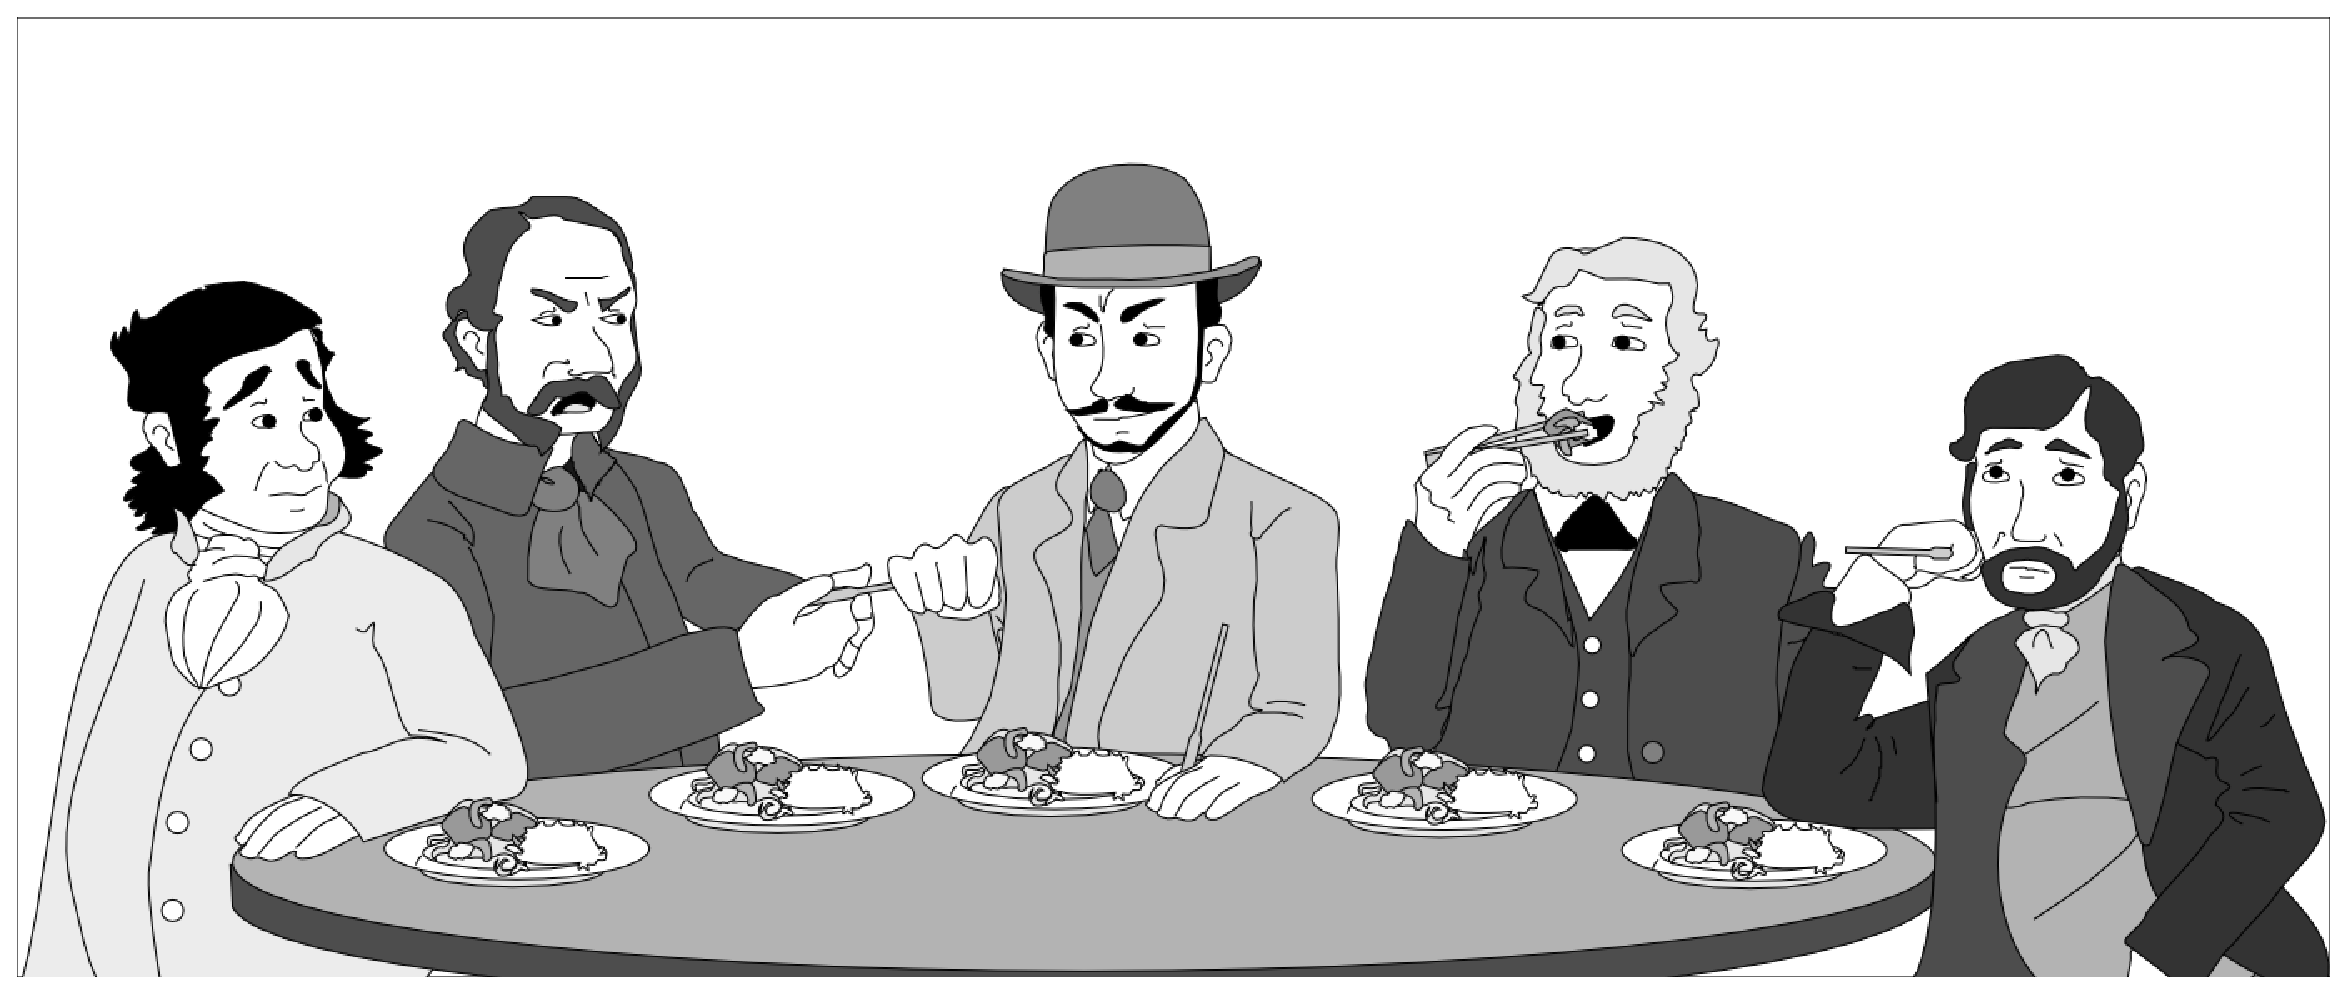
\includegraphics{cartoons/Dining-philosophers}}
\caption{Partial Starvation Is Also Bad}
\ContributedBy{Figure}{fig:cpu:Partial Starvation Is Also Bad}{Melissa Broussard}
\end{figure*}

목표는 말 그대로 기아를 방지할 수 있는 알고리즘을 만드는 것입니다.
가능한 한가지 기아 시나리오는 모든 철학자가 각자의 왼쪽 포크를 동시에 집어드는
경우입니다.
이들 중 누구도 그들이 식사를 끝내기 전까지는 자신의 포크를 내려놓지 않을
것이므로, 그리고 이들 중 누구도 이들 중 한명이라도 식사를 끝내기 전까지는
두번째 포크를 갖지 못할 것이므로, 이들은 모두 굶게 됩니다.
최소 한명의 철학자를 식사할 수 있게 하는 것만으로는 충분치 않음을 알아 두시기
바랍니다.
Figure~\ref{fig:cpu:Partial Starvation Is Also Bad} 가 보이듯, 오직 소수의
철학자가 기아에 빠지는 것조차도 방지되어야 합니다.

\iffalse

The object is to construct an algorithm that, quite literally,
prevents starvation.
One starvation scenario would be if all of the philosophers picked up
their leftmost forks simultaneously.
Because none of them will put down their fork until after they finished
eating, and because none of them may pick up their second fork until at
least one of them has finished eating, they all starve.
Please note that it is not sufficient to allow at least one philosopher
to eat.
As Figure~\ref{fig:cpu:Partial Starvation Is Also Bad}
shows, starvation of even a few of the philosophers is to be avoided.

\fi

\begin{figure}[tb]
\centering
\includegraphics[scale=.7]{SMPdesign/DiningPhilosopher5TB}
\caption{Dining Philosophers Problem, Textbook Solution}
\ContributedBy{Figure}{fig:SMPdesign:Dining Philosophers Problem, Textbook Solution}{Kornilios Kourtis}
\end{figure}

\pplsur{Edsger W.}{Dijkstra} 의 해결책은 1980년대 말 또는 1990년대 초에는
적절치 못하게 된, 무시할만한 통신 딜레이라는 가정을 적용하면 잘 동작하는 전역
세마포어를 사용했습니다.\footnote{
	2021년의 시각에서 Dijkstra 를 모욕하기는 너무도 쉽습니다, 50년이나 지난
	이야기니까요.
	여전히 Dijkstra 를 모욕해야 한다고 느끼신다면, 저는 무언가를 출판하고,
	50년을 기다린 후, \emph{여러분의} 아이디어가 그 시간동안의 시험을
	얼마나 잘 버텨냈는지 보라는 조언을 하겠습니다.}
보다 최신의 해결책은
Figure~\ref{fig:SMPdesign:Dining Philosophers Problem, Textbook Solution}
에 보인 것처럼 포크에 수를 매기는 것입니다.
각 철학자는 그 또는 그녀의 접시 옆에 있는 더 낮은 수를 가지는 포크를 집고,
그다음 다음 포크를 집습니다.
따라서, 이 그림에서 가장 위쪽에 앉은 철학자는 왼쪽 포크를 먼저 집어들고, 이어서
오른쪽 포크를 집어드는데, 나머지 철학자들은 각자의 오른쪽 포크를 먼저
집어듭니다.
두명의 철학자들이 포크~1 을 먼저 집어들려고 노력할 것이므로, 그리고 이 두
철학자들 중 한명만이 성공할 것이므로, 네명의 철학자에게 다섯개의 포크가 사용
가능하게 될 겁니다.
이 네명의 철학자 중 최소 한명은 두개의 포크를 가지게 될거고 따라서 식사를 할 수
있습니다.

\iffalse

\pplsur{Edsger W.}{Dijkstra}'s solution used a global semaphore,
which works fine assuming
negligible communications delays, an assumption that became invalid
in the late 1980s or early 1990s.\footnote{
	It is all too easy to denigrate Dijkstra from the viewpoint
	of the year 2021, more than 50 years after the fact.
	If you still feel the need to denigrate Dijkstra, my advice
	is to publish something, wait 50 years, and then see
	how well \emph{your} ideas stood the test of time.}
More recent solutions number the forks as shown in
Figure~\ref{fig:SMPdesign:Dining Philosophers Problem, Textbook Solution}.
Each philosopher picks up the lowest-numbered fork next to his or her
plate, then picks up the other fork.
The philosopher sitting in the uppermost position in the diagram thus
picks up the leftmost fork first, then the rightmost fork, while the
rest of the philosophers instead pick up their rightmost fork first.
Because two of the philosophers will attempt to pick up fork~1 first,
and because only one of those two philosophers will succeed,
there will be five forks available to four philosophers.
At least one of these four will have two forks, and will thus be able
to eat.

\fi

이 자원에 숫자를 매기고 그 숫자 순서대로 자원을 획득하는 일반적인 기법은 데드락
방지 기법으로 널리 사용되었습니다.
하지만, 모두가 배고픈데 한번에 단 한명의 철학자만이 식사를 하는 상황이 초래되는
사건의 연속을 쉽게 상상해 볼 수 있습니다:

\begin{enumerate}
    \item P2 가 포크~1 을 집어들어, P1 이 포크를 집는 걸 방지합니다.
    \item P3 가 포크~2 를 집어듭니다.
    \item P4 가 포크~3 를 집어듭니다.
    \item P5 가 포크~4 를 집어듭니다.
    \item P5 가 포크~5 를 집어들고 식사를 합니다.
    \item P5 가 포크~4 와~5 를 내려놓습니다.
    \item P4 가 포크~4 를 집어들고 식사를 합니다.
\end{enumerate}

요약하자면, 이 알고리즘은 동시에 두 철학자가 식사를 하기 충분한 것 이상의
포크가 존재함에도 불구하고 모든 철학자가 배고플 때에도 한번에 하나의 철학자만
식사를 하는 상황을 초래할 수 있습니다.
이보다 더 잘할 수 있어야 합니다!

\iffalse

This general technique of numbering resources and acquiring them in
numerical order is heavily used as a deadlock-prevention technique.
However, it is easy to imagine a sequence of events that will result
in only one philosopher eating at a time even though all are hungry:

\begin{enumerate}
    \item P2 picks up fork~1, preventing P1 from taking a fork.
    \item P3 picks up fork~2.
    \item P4 picks up fork~3.
    \item P5 picks up fork~4.
    \item P5 picks up fork~5 and eats.
    \item P5 puts down forks~4 and~5.
    \item P4 picks up fork~4 and eats.
\end{enumerate}

In short, this algorithm can result in only one philosopher eating at
a given time, even when all five philosophers are hungry,
despite the fact that there are more than enough forks for two
philosophers to eat concurrently.
It should be possible to do better than this!

\fi

\begin{figure}[tb]
\centering
\includegraphics[scale=.7]{SMPdesign/DiningPhilosopher4part-b}
\caption{Dining Philosophers Problem, Partitioned}
\ContributedBy{Figure}{fig:SMPdesign:Dining Philosophers Problem, Partitioned}{Kornilios Kourtis}
\end{figure}

한가지 해결책이
Figure~\ref{fig:SMPdesign:Dining Philosophers Problem, Partitioned}
에 그려져 있는데, 이 파티셔닝 기법을 더 잘 보이기 위해 다섯명이 아닌 네명의
철학자만 포함하고 있습니다.
여기서 위쪽과 오른쪽의 철학자들은 한쌍의 포크를 공유하며, 아래쪽과 왼쪽의
철학자는 다른 한쌍의 포크를 공유합니다.
만약 모든 철학자들이 동시에 배고파지면, 최소 두명은 항상 동시에 식사를 할 수
있습니다.
또한, 그림에 보여져 있듯이, 이 포크들은 이제 한쌍으로 묶여있을 수 있어서 두개씩
동시에 집어지고 내려놓아질 수 있게 되어, 획득과 해제 알고리즘을 단순화
시킵니다.

\iffalse

One approach is shown in
Figure~\ref{fig:SMPdesign:Dining Philosophers Problem, Partitioned},
which includes four philosophers rather than five to better illustrate the
partition technique.
Here the upper and rightmost philosophers share a pair of forks,
while the lower and leftmost philosophers share another pair of forks.
If all philosophers are simultaneously hungry, at least two will
always be able to eat concurrently.
In addition, as shown in the figure, the forks can now be bundled
so that the pair are picked up and put down simultaneously, simplifying
the acquisition and release algorithms.

\fi

\QuickQuiz{
	이 Dining Philosophers 문제에 더 나은 해결책이 있을까요?

	\iffalse

	Is there a better solution to the Dining
	Philosophers Problem?

	\fi

}\QuickQuizAnswer{
	그런 향상된 해결책 하나가
	Figure~\ref{fig:SMPdesign:Dining Philosophers Problem, Fully Partitioned}
	에 보여져 있는데, 단순히 철학자들에게 추가의 다섯개 포크를 제공하는
	것입니다.
	모든 다섯명의 철학자가 이제 동시에 식사를 할 수 있고, 어떤 철학자도
	다른 누군가를 기다릴 필요가 없습니다.
	또한, 이 방법은 무척 향상된 재앙 통제를 제공합니다.

	\iffalse

	One such improved solution is shown in
	Figure~\ref{fig:SMPdesign:Dining Philosophers Problem, Fully Partitioned},
	where the philosophers are simply provided with an additional
	five forks.
	All five philosophers may now eat simultaneously, and there
	is never any need for philosophers to wait on one another.
	In addition, this approach offers greatly improved disease control.

	\fi

\begin{figure}[tb]
\centering
\includegraphics[scale=.7]{SMPdesign/DiningPhilosopher5PEM}
\caption{Dining Philosophers Problem, Fully Partitioned}
\QContributedBy{Figure}{fig:SMPdesign:Dining Philosophers Problem, Fully Partitioned}{Kornilios Kourtis}
\end{figure}

	이 해결책은 누군가에겐 속임수처럼 보일 수도 있겠습니다만, 이런 종류의
	``속임수'' 가 많은 동시성 문제에 있어 좋은 해결책을 찾기 위한
	열쇠입니다.

	\iffalse

	This solution might seem like cheating to some, but such
	``cheating'' is key to finding good solutions to many
	concurrency problems.

	\fi

}\QuickQuizEnd

이는 ``수평 병렬성''~\cite{Inman85} 또는 ``데이터 병렬성'' 의 한 예로, 이
철학자들 쌍 간에는 어떤 의존성이 없기 때문에 그렇게 이름지어졌습니다.
수평적으로 병렬인 데이터 처리 시스템에서, 데이터의 특정 항목은 복사된
소프트웨어 컴포넌트들 중 하나에 의해서만 처리될 겁니다.

\iffalse

This is an example of ``horizontal parallelism''~\cite{Inman85}
or ``data parallelism'',
so named because there is no dependency among the pairs of philosophers.
In a horizontally parallel data-processing system, a given item of data
would be processed by only one of a replicated set of software
components.

\fi

\QuickQuiz{
	그리고 어떤 의미에서 이 ``수평적 병렬성'' 은 ``수평적'' 이라고 불릴 수
	있는 건가요?

	\iffalse

	And in just what sense can this ``horizontal parallelism'' be
	said to be ``horizontal''?

	\fi

}\QuickQuizAnswer{
	Inman 은 일반적으로 어플리케이션이 꼭대기에, 그리고 하드웨어 연결부가
	바닥에, 수직으로 그려지는 프로토콜 스택을 가지고 일하고 있었습니다.
	데이터는 이 스택의 위에서 아래로 흐릅니다.
	``수평적 병렬성'' 은 패킷을 다른 네트워크 연결부로부터 병렬로 처리하는
	반면, ``수직 병렬성'' 은 주어진 패킷을 다른 프로토콜 처리 단계로 동시에
	처리합니다.

	``수직 병렬성'' 은 또한 ``파이프라이닝'' 이라고도 불립니다.

	\iffalse

	Inman was working with protocol stacks, which are normally
	depicted vertically, with the application on top and the
	hardware interconnect on the bottom.
	Data flows up and down this stack.
	``Horizontal parallelism'' processes packets from different network
	connections in parallel, while ``vertical parallelism''
	handles different protocol-processing steps for a given
	packet in parallel.

	``Vertical parallelism'' is also called ``pipelining''.

	\fi

}\QuickQuizEnd

\subsection{Double-Ended Queue}
\label{sec:SMPdesign:Double-Ended Queue}

Double-ended queue 는 양 끝을 통해 추가되거나 제거될 수 있는 원소들의 리스트를
갖는 데이터 구조입니다~\cite{Knuth73}.
락 기반의 구현으로는 double-ended queue 의 양 끝단에서의 동시적 운용이
어려움으로 알려져 있습니다~\cite{DanGrossman2007TMGCAnalogy}.
이 섹션은 파티셔닝 설계 전략이 어떻게 합리적으로 간단한 구현에 이르게 할 수
있는지 보이고, 뒤따르는 섹션들에서는 세개의 범용 접근법을 봅니다.

\iffalse

A double-ended queue is a data structure containing a list of elements
that may be inserted or removed from either end~\cite{Knuth73}.
It has been claimed that a lock-based implementation permitting
concurrent operations on both ends of the double-ended queue is
difficult~\cite{DanGrossman2007TMGCAnalogy}.
This section shows how a partitioning design strategy can result
in a reasonably simple implementation, looking at three
general approaches in the following sections.

\fi

\subsubsection{Left- and Right-Hand Locks}
\label{sec:SMPdesign:Left- and Right-Hand Locks}

\begin{figure}[tb]
\centering
\resizebox{3in}{!}{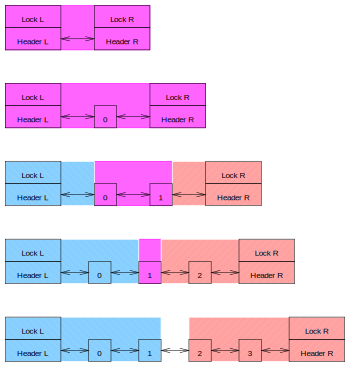
\includegraphics{SMPdesign/lockdeq}}
\caption{Double-Ended Queue With Left- and Right-Hand Locks}
\label{fig:SMPdesign:Double-Ended Queue With Left- and Right-Hand Locks}
\end{figure}

간단해 보이는 한가지 전략은 왼쪽 끝으로의 enqueue 와 dequeue 오퍼레이션을 위한
왼쪽 락과 오른쪽 끝으로의 오퍼레이션들을 위한 오른쪽 락을 갖는 doubly linked
list 를 사용하는 것으로,
Figure~\ref{fig:SMPdesign:Double-Ended Queue With Left- and Right-Hand Locks}
에 보이는 것과 같습니다.
하지만, 이 방법의 문제는 이 리스트에 네개 미만의 원소만이 존재할 때에는 이 두
락의 도메인이 겹친다는 것입니다.
이 겹침은 어떤 원소를 제거하는 것이 그 원소만이 아니라 그것의 왼쪽과 오른쪽
이웃 원소에게도 영향을 끼친다는 사실 때문입니다.
이 도메인들은 이 그림에 색깔로 표시되어 있는데, 아래쪽으로의 줄무늬를 가진
파랑은 왼쪽 락의 도메인을, 위쪽으로의 줄무늬를 가진 빨강은 오른쪽 락의
도메인을, 그리고 (줄무늬가 없는) 보라색은 겹치는 도메인을 표시합니다.
이 방식으로 동작하는 알고리즘을 만드는 것도 가능하지만, 다섯개 미만이 아닌 특수
경우들이 존재한다는 사실은 커다랗고 빨간 경고등을 띄우는데, 이 리스트의 다른
끝쪽에서의 동시의 행동들이 이 queue 를 언제든 하나의 특수 경우에서 다른 경우로
바꿀 수 있다는 점에서 특히 그렇습니다.
다른 설계를 고려하는 게 훨씬 나을 겁니다.

\iffalse

One seemingly straightforward approach would be to use a doubly
linked list with a left-hand lock
for left-hand-end enqueue and dequeue operations along with a right-hand
lock for right-hand-end operations, as shown in
Figure~\ref{fig:SMPdesign:Double-Ended Queue With Left- and Right-Hand Locks}.
However, the problem with this approach is that the two locks'
domains must overlap when there are fewer than four elements on the
list.
This overlap is due to the fact that removing any given element affects
not only that element, but also its left- and right-hand neighbors.
These domains are indicated by color in the figure, with blue
with downward stripes indicating
the domain of the left-hand lock, red with upward stripes
indicating the domain of the right-hand
lock, and purple (with no stripes) indicating overlapping domains.
Although it is possible to create an algorithm that works this way,
the fact that it has no fewer than five special cases should raise
a big red flag, especially given that concurrent activity at the other
end of the list can shift the queue from one special case to another
at any time.
It is far better to consider other designs.

\fi

\subsubsection{Compound Double-Ended Queue}
\label{sec:SMPdesign:Compound Double-Ended Queue}

\begin{figure}[tb]
\centering
\resizebox{3in}{!}{\includegraphics{SMPdesign/lockdeqpair}}
\caption{Compound Double-Ended Queue}
\label{fig:SMPdesign:Compound Double-Ended Queue}
\end{figure}

겹치지 않는 락 도메인을 강제하기 위한 한가지 방법이
Figure~\ref{fig:SMPdesign:Compound Double-Ended Queue}
에 보여져 있습니다.
두개의 double-ended queue 들이 동시에 동작하는데, 각각 자신의 락으로
보호됩니다.
이는 원소들이 결국은 한쪽 double-ended queue 에서 다른 쪽으로 옮겨져야 하며,
이때는 양쪽 락이 모두 잡혀야만 함을 의미합니다.
데드락을 방지하기 위해 간단한 락 계층이 사용될 수 있는데, 예를 들면 오른쪽 락을
잡기 전에 항상 왼쪽 락을 잡는 겁니다.
이러면 우리는 조건 없이 왼쪽 queue 에 원소를 왼쪽 집어넣기하고 오른쪽 queue 에
원소를 오른쪽 집어넣기를 할 수 있으므로, 같은 double-ended queue 에 두개의 락을
적용하는 것보다는 훨씬 간단할 것입니다.
비어있는 queue 에서 꺼내기를 하려 할 때 주요한 복잡도가 나타나는데, 이 경우에는
다음과 같은 처리가 필요합니다:

\iffalse

One way of forcing non-overlapping lock domains is shown in
Figure~\ref{fig:SMPdesign:Compound Double-Ended Queue}.
Two separate double-ended queues are run in tandem, each protected by
its own lock.
This means that elements must occasionally be shuttled from one of
the double-ended queues to the other, in which case both locks must
be held.
A simple lock hierarchy may be used to avoid deadlock, for example,
always acquiring the left-hand lock before acquiring the right-hand lock.
This will be much simpler than applying two locks to the same
double-ended queue, as we can unconditionally left-enqueue elements
to the left-hand queue and right-enqueue elements to the right-hand
queue.
The main complication arises when dequeuing from an empty queue, in
which case it is necessary to:

\fi

\begin{enumerate}
\item	오른쪽 락을 잡고 있다면, 이를 해제하고 왼쪽 락을 잡습니다.
\item	오른쪽 락을 잡습니다.
\item	두 queue 에 원소를 고르게 분배시킵니다.
\item	제거하려는 원소가 있다면 제거합니다.
\item	두 락을 모두 해제합니다.

\iffalse

\item	If holding the right-hand lock, release it and acquire the
	left-hand lock.
\item	Acquire the right-hand lock.
\item	Rebalance the elements across the two queues.
\item	Remove the required element if there is one.
\item	Release both locks.

\fi

\end{enumerate}

\QuickQuiz{
	이 compound double-ended queue 구현에서는, 이 락을 해제하고 재획득 하는
	동안에 이 queue 가 비어있지 않게 되면 어떡해야 하죠?

	\iffalse

	In this compound double-ended queue implementation, what should
	be done if the queue has become non-empty while releasing
	and reacquiring the lock?

	\fi

}\QuickQuizAnswer{
	이 경우에는, 그냥 이 비어있지 않은 큐에서 원소를 제거하고, 두 락을
	해제하고, 리턴하면 됩니다.

	\iffalse

	In this case, simply dequeue an item from the non-empty
	queue, release both locks, and return.

	\fi

}\QuickQuizEnd

이 결과로 나오는 코드는 (\path{locktdeq.c}) 상당히 간단합니다.
원소 재분배 오퍼레이션은 주어진 원소를 두 queue 사이에서 어느 쪽으로든 옮길
수도 있어서, 시간을 낭비하고, 최적의 성능을 위해선 워크로드 종속적 휴리스틱을
필요로 할 수도 있습니다.
이게 어떤 경우에는 최선의 방법이 될수도 있겠습니다만, 알고리즘을 더 큰 결정성을
가지고 시도해 보는것도 흥미로울 겁니다.

\iffalse

The resulting code (\path{locktdeq.c}) is quite straightforward.
The rebalancing operation might well shuttle a given element back
and forth between the two queues, wasting time and possibly requiring
workload-dependent heuristics to obtain optimal performance.
Although this might well be the best approach in some cases, it is
interesting to try for an algorithm with greater determinism.

\fi

\subsubsection{Hashed Double-Ended Queue}
\label{sec:SMPdesign:Hashed Double-Ended Queue}

데이터 구조를 결정론적으로 쪼개는 가장 효과적이고도 가장 간단한 방법은
해싱입니다.
각 원소에 이 리스트에서의 그것의 위치에 기반한 숫자를 부여해서 비어있는 queue
에 왼쪽으로 들어온 첫번째 원소는 0으로 수가 부여되고 비어있는 queue 에
오른쪽으로 들어온 첫번째 원소는 1이라는 수가 부여되는 식으로 double-ended
queue 를 간단히 해싱하는게 가능합니다.
왼쪽으로 들어오는 원소들은 계속해서 작아지는 수를 부여받고 ($-1$, $-2$, $-3$,
\ldots), 오른쪽으로 들어오는 원소들은 계속해서 증가하는 수를 부여받습니다 (2,
3, 4, \ldots).
핵심은, 이 숫자가 이 queue 에서의 위치를 암시하므로, 해당 원소의 수를 정말로
표현할 필요는 없다는 겁니다.

\iffalse

One of the simplest and most effective ways to deterministically
partition a data structure is to hash it.
It is possible to trivially hash a double-ended queue by assigning
each element a sequence number based on its position in the list,
so that the first element left-enqueued into an empty queue is numbered
zero and the first element right-enqueued into an empty queue is numbered
one.
A series of elements left-enqueued into an otherwise-idle queue would
be assigned decreasing numbers ($-1$, $-2$, $-3$, \ldots), while a series of
elements right-enqueued into an otherwise-idle queue would be assigned
increasing numbers (2, 3, 4, \ldots).
A key point is that it is not necessary to actually represent a given
element's number, as this number will be implied by its position in
the queue.

\fi

\begin{figure}[tb]
\centering
\resizebox{3in}{!}{\includegraphics{SMPdesign/lockdeqhash}}
\caption{Hashed Double-Ended Queue}
\label{fig:SMPdesign:Hashed Double-Ended Queue}
\end{figure}

이 방법에서는, 우리는 왼쪽 인덱스를 보호하기 위해 하나의 락을 할당하고, 오른쪽
인덱스를 위해 또다른 락을, 그리고 각 해쉬 체인을 위해 또하나의 락을 사용합니다.
Figure~\ref{fig:SMPdesign:Hashed Double-Ended Queue} 가 네개의 해쉬 체인이
있다는 가정 하에 이로 인해 만들어지는 데이터 구조를 보입니다.
락 도메인은 겹치지 않으며, 데드락은 체인 락 전에 인덱스 락을 획득함으로써
회피되며, 특정 타입의 (인덱스 또는 체인) 락은 한번에 두개 이상 획득하지
않습니다.

\iffalse

Given this approach, we assign one lock to guard the left-hand index,
one to guard the right-hand index, and one lock for each hash chain.
Figure~\ref{fig:SMPdesign:Hashed Double-Ended Queue} shows the resulting
data structure given four hash chains.
Note that the lock domains do not overlap, and that deadlock is avoided
by acquiring the index locks before the chain locks, and by never
acquiring more than one lock of a given type (index or chain) at a time.

\fi

\begin{figure}[tb]
\centering
\resizebox{3in}{!}{
\includegraphics{SMPdesign/lockdeqhash1R}}
\caption{Hashed Double-Ended Queue After Insertions}
\label{fig:SMPdesign:Hashed Double-Ended Queue After Insertions}
\end{figure}

각 해쉬 체인은 그 자체로 double-ended queue 이며, 이 예에서는 각각이 네개의
원소씩을 쥐고 있습니다.
Figure~\ref{fig:SMPdesign:Hashed Double-Ended Queue After Insertions}
의 가장 위쪽은 하나의 원소가 (``R$_1$'') 오른쪽으로 넣어지고, 해쉬 체인~2 를
참조하게끔 증가된 오른쪽 인덱스를 갖게 된 후의 상태를 보입니다.
이 그림의 가운데 부분은 세개의 원소가 추가적으로 오른쪽으로 넣어진 후의 상태를
보입니다.
보시다시피, 인덱스들은 각자의 초기 상태로 되돌아가져 있습니다
(Figure~\ref{fig:SMPdesign:Hashed Double-Ended Queue}를 보세요), 하지만 각 해시
체인은 이제 비어 있습니다.
이 그림의 아래쪽은 세개의 추가적인 원소가 왼쪽으로 들어오고 또하나의 원소가
오른쪽으로 들어온 후의 상태를 보입니다.

Figure~\ref{fig:SMPdesign:Hashed Double-Ended Queue After Insertions} 에 보인
마지막 상태로부터, 왼쪽 dequeue 오퍼레이션은 원소 ``L$_{-2}$'' 를 리턴하고,
왼쪽 인덱스가 해쉬 체인~2 를 참조하는대로 둘 것이며, 이 체인은 단 하나의
원소만을 (``R$_2$'') 가지고 있게 됩니다.
이 상태에서, 왼쪽 enqueue 가 오른쪽 enqueue 와 동시에 수행되면 락 경쟁이 발생할
겁니다만, 그런 경쟁 상태의 확률은 더 큰 해쉬 테이블을 사용함으로써 무척 낮은
수준으로 줄일 수 있습니다.

\iffalse

Each hash chain is itself a double-ended queue, and in this example,
each holds every fourth element.
The uppermost portion of
Figure~\ref{fig:SMPdesign:Hashed Double-Ended Queue After Insertions}
shows the state after a single element (``R$_1$'') has been
right-enqueued, with the right-hand index having been incremented to
reference hash chain~2.
The middle portion of this same figure shows the state after
three more elements have been right-enqueued.
As you can see, the indexes are back to their initial states
(see Figure~\ref{fig:SMPdesign:Hashed Double-Ended Queue}), however,
each hash chain is now non-empty.
The lower portion of this figure shows the state after three additional
elements have been left-enqueued and an additional element has been
right-enqueued.

From the last state shown in
Figure~\ref{fig:SMPdesign:Hashed Double-Ended Queue After Insertions},
a left-dequeue operation would return element ``L$_{-2}$'' and leave
the left-hand index referencing hash chain~2, which would then
contain only a single element (``R$_2$'').
In this state, a left-enqueue running concurrently with a right-enqueue
would result in lock contention, but the probability of such contention
can be reduced to arbitrarily low levels by using a larger hash table.

\fi

\begin{figure}[tb]
\centering
\resizebox{1.5in}{!}{
\includegraphics{SMPdesign/lockdeqhashlots}}
\caption{Hashed Double-Ended Queue With 16 Elements}
\label{fig:SMPdesign:Hashed Double-Ended Queue With 16 Elements}
\end{figure}

Figure~\ref{fig:SMPdesign:Hashed Double-Ended Queue With 16 Elements}
는 16개의 원소가 네개 해쉬 버킷 기반의 병렬 double-ended queue 에 어떻게 관리될
지 보입니다.
아랫단의 단일 락 기반 double-ended queue 각각은 전체 병렬 double-ended queue 의
1/4 조각을 갖습니다.

\iffalse

Figure~\ref{fig:SMPdesign:Hashed Double-Ended Queue With 16 Elements}
shows how 16 elements would be organized in a four-hash-bucket
parallel double-ended queue.
Each underlying single-lock double-ended queue holds a one-quarter
slice of the full parallel double-ended queue.

\fi

\begin{listing}[tbp]
\input{CodeSamples/SMPdesign/lockhdeq@struct_pdeq.fcv}
\caption{Lock-Based Parallel Double-Ended Queue Data Structure}
\label{lst:SMPdesign:Lock-Based Parallel Double-Ended Queue Data Structure}
\end{listing}

Listing~\ref{lst:SMPdesign:Lock-Based Parallel Double-Ended Queue Data Structure}
은 평범하게 락으로 관리되는 double-ended-queue 구현을 제공하는 \co{struct deq}
가 존재한다는 가정 하에 앞에서 이야기한 것에 연관되는 C-언어 데이터 구조를
보입니다.
\begin{fcvref}[ln:SMPdesign:lockhdeq:struct_pdeq]
이 데이터 구조는 라인~\lnref{llock} 에 왼쪽 락을, 라인~\lnref{lidx} 에 왼쪽
인덱스를, 라인~\lnref{rlock} 에 오른쪽 락을 (실제 구현에서는 캐쉬라인 사이즈로
정렬된), 라인~\lnref{ridx} 에 오른쪽 인덱스를, 그리고 마지막으로,
라인~\lnref{bkt} 에 간단한 락 기반 double-ended queue 의 배열을 가지고
있습니다.
고성능 구현체는 거짓 공유를 피하기 위해 패딩이나 특수한 정렬 지시어 등을 사용할
겁니다.
\end{fcvref}

\iffalse

Listing~\ref{lst:SMPdesign:Lock-Based Parallel Double-Ended Queue Data Structure}
shows the corresponding C-language data structure, assuming an
existing \co{struct deq} that provides a trivially locked
double-ended-queue implementation.
\begin{fcvref}[ln:SMPdesign:lockhdeq:struct_pdeq]
This data structure contains the left-hand lock on line~\lnref{llock},
the left-hand index on line~\lnref{lidx}, the right-hand lock on line~\lnref{rlock}
(which is cache-aligned in the actual implementation),
the right-hand index on line~\lnref{ridx}, and, finally, the hashed array
of simple lock-based double-ended queues on line~\lnref{bkt}.
A high-performance implementation would of course use padding or special
alignment directives to avoid false sharing.
\end{fcvref}

\fi

\begin{listing}[tbp]
\input{CodeSamples/SMPdesign/lockhdeq@pop_push.fcv}
\caption{Lock-Based Parallel Double-Ended Queue Implementation}
\label{lst:SMPdesign:Lock-Based Parallel Double-Ended Queue Implementation}
\end{listing}

Listing~\ref{lst:SMPdesign:Lock-Based Parallel Double-Ended Queue Implementation}
(\path{lockhdeq.c})
은 enqueue 와 dequeue 함수의 구현을 보입니다.\footnote{
	어떤 언어를 사용해서든 다양한 형태의 구현을 만들 수 있겠습니다만, 그건
	독자 여러분의 연습 문제로 남겨 두겠습니다.}
이야기는 왼쪽 오퍼레이션들에 집중할텐데, 오른쪽 오퍼레이션들은 쉽게 왼쪽의
것들로부터 나올 것이기 때문입니다.

\begin{fcvref}[ln:SMPdesign:lockhdeq:pop_push:popl]
\Clnrefrange{b}{e} 는 왼쪽 dequeue 를 하고 가능하면 원소를, 그렇지 않다면
\co{NULL} 을 리턴하는 \co{pdeq_pop_l()} 을 보입니다.
라인~\lnref{acq} 는 왼쪽 스핀락을 획득하고, 라인~\lnref{idx} 는 dequeue 될
인덱스를 계산합니다.
라인~\lnref{deque} 는 이 원소를 꺼내고, 라인~lnref{check} 에서 이 결과가
\co{NULL} 이 아닐 것으로 판명되면, 라인~\lnref{rel} 에서 락을 해제하고,
마지막으로 라인~\lnref{return} 에서 거기 원소가 있었다면 그것을, 아니면
\co{NULL} 을 리턴합니다.
\end{fcvref}

\iffalse

Listing~\ref{lst:SMPdesign:Lock-Based Parallel Double-Ended Queue Implementation}
(\path{lockhdeq.c})
shows the implementation of the enqueue and dequeue functions.\footnote{
	One could easily create a polymorphic implementation in any
	number of languages, but doing so is left as an exercise for
	the reader.}
Discussion will focus on the left-hand operations, as the right-hand
operations are trivially derived from them.

\begin{fcvref}[ln:SMPdesign:lockhdeq:pop_push:popl]
\Clnrefrange{b}{e} show \co{pdeq_pop_l()},
which left\-/dequeues and returns
an element if possible, returning \co{NULL} otherwise.
Line~\lnref{acq} acquires the left-hand spinlock,
and line~\lnref{idx} computes the
index to be dequeued from.
Line~\lnref{deque} dequeues the element, and,
if line~\lnref{check} finds the result to be
non-\co{NULL}, line~\lnref{record} records the new left-hand index.
Either way, line~\lnref{rel} releases the lock, and,
finally, line~\lnref{return} returns
the element if there was one, or \co{NULL} otherwise.
\end{fcvref}

\fi

\begin{fcvref}[ln:SMPdesign:lockhdeq:pop_push:pushl]
\Clnrefrange{b}{e} 는 특정 원소를 왼쪽으로 enqueue 하는 \co{pdeq_push_l()} 을
보입니다.
라인~\lnref{acq} 는 왼쪽 락을 획득하고, 라인~\lnref{idx} 에서 왼쪽 인덱스를
잡습니다.
라인~\lnref{enque} 는 이 원소를 이 왼쪽 인덱스로 가리켜지는 double-ended queue
에 왼쪽으로 enqueue gkqslek.
라인~\lnref{update} 는 이어서 이 왼쪽 인덱스를 업데이트 하고 라인~\lnref{rel}
에서 이 락을 해제합니다.
\end{fcvref}

앞에서도 이야기 했듯, 오른쪽 오퍼레이션들은 왼쪽의 것들과 완전히 비슷하므로,
그것들의 분석은 독자 여러분의 연습 문제로 남겨 둡니다.

\iffalse

\begin{fcvref}[ln:SMPdesign:lockhdeq:pop_push:pushl]
\Clnrefrange{b}{e} show \co{pdeq_push_l()},
which left-enqueues the specified
element.
Line~\lnref{acq} acquires the left-hand lock,
and line~\lnref{idx} picks up the left-hand
index.
Line~\lnref{enque} left-enqueues the specified element
onto the double-ended queue
indexed by the left-hand index.
Line~\lnref{update} then updates the left-hand index
and line~\lnref{rel} releases the lock.
\end{fcvref}

As noted earlier, the right-hand operations are completely analogous
to their left-handed counterparts, so their analysis is left as an
exercise for the reader.

\fi

\QuickQuiz{
	해쉬 기반의 double-ended queue 는 좋은 해결책일까요?
	왜 그렇고 왜 그렇지 않을까요?

	\iffalse

	Is the hashed double-ended queue a good solution?
	Why or why not?

	\fi

}\QuickQuizAnswer{
	여기 답변하는 최선의 방법은 여러개의 다른 멀티프로세서 시스템에서
	\path{lockhdeq.c} 를 수행해 보는 것이며, 여러분이 가능한 시간 내에
	그렇게 할 것을 장려합니다.
	걱정을 할 수 있는 한가지 이유는 이 구현에서 각 오퍼레이션은 하나가 아닌
	두개의 락을 획득해야 한다는 것입니다.

	잘 설계된 첫번째 성능 연구가 예로 들어질 겁니다.\footnote{
		Dalessandro 등의
		연구~\cite{LukeDalessandro:2011:ASPLOS:HybridNOrecSTM:deque}
		와 Dice 등의 연구~\cite{DavidDice:2010:SCA:HTM:deque} 는 훌륭한
		시작 지점이 될 겁니다.}
	순차적 구현과의 비교도 잊지 마십시오!

	\iffalse

	The best way to answer this is to run \path{lockhdeq.c} on
	a number of different multiprocessor systems, and you are
	encouraged to do so in the strongest possible terms.
	One reason for concern is that each operation on this
	implementation must acquire not one but two locks.
	% Getting about 500 nanoseconds per element when used as
	% a queue on a 4.2GHz Power system.  This is roughly the same as
	% the version covered by a single lock.  Sequential (unlocked
	% variant is more than an order of magnitude faster!

	The first well-designed performance study will be cited.\footnote{
		The studies by Dalessandro
		et al.~\cite{LukeDalessandro:2011:ASPLOS:HybridNOrecSTM:deque}
		and Dice et al.~\cite{DavidDice:2010:SCA:HTM:deque} are
		excellent starting points.}
	Do not forget to compare to a sequential implementation!

	\fi

}\QuickQuizEnd

\subsubsection{Compound Double-Ended Queue Revisited}
\label{sec:SMPdesign:Compound Double-Ended Queue Revisited}

이 섹션은 조합된 double-ended queue 를 비어 있지 않은 queue 에서 이제 비어 있는
queue 로 모든 원소를 옮기는 간단한 균형 맞추기를 사용하는 방법으로 다시
풀어봅니다.

\iffalse

This section revisits the compound double-ended queue, using a trivial
rebalancing scheme that moves all the elements from the non-empty
queue to the now-empty queue.

\fi

\QuickQuiz{
	빈 queue 로 \emph{모든} 원소를 옮긴다구요?
	이 미친 해결책이 대체 어떤 세상에서는 최적인거죠???

	\iffalse

	Move \emph{all} the elements to the queue that became empty?
	In what possible universe is this brain-dead solution in any
	way optimal???

	\fi

}\QuickQuizAnswer{
	데이터 흐름의 방향이 가끔씩만 바뀌는 경우에 최적입니다.
	이 double-ended queue 가 동시에 양 끝에서 비워지는 경우엔 물론 무척
	안좋은 선택일 겁니다.
	이는 물론 다른 질문을 떠오르게 하는데, 양끝에서 동시에 비우기를 하는건
	대체 어떤 세상에서 합리적인 일이겠냐는 겁니다.
	이 질문에 대한 가능한 답 중 하나는 work stealing queue 입니다.

	\iffalse

	It is optimal in the case where data flow switches direction only
	rarely.
	It would of course be an extremely poor choice if the double-ended
	queue was being emptied from both ends concurrently.
	This of course raises another question, namely, in what possible
	universe emptying from both ends concurrently would be a reasonable
	thing to do.
	Work-stealing queues are one possible answer to this question.

	\fi

}\QuickQuizEnd

앞의 섹션에서 보인 해쉬 기반 구현과 대조적으로, 이 조합 구현은 락도 어토믹
오퍼레이션도 사용하지 않는 순차적 구현의 double-ended queue 위에서 구현될
겁니다.

\iffalse

In contrast to the hashed implementation presented in
the previous section, the compound implementation will build on
a sequential implementation of a double-ended queue that uses
neither locks nor atomic operations.

\fi

\begin{listing}[tbp]
\input{CodeSamples/SMPdesign/locktdeq@pop_push.fcv}
\caption{Compound Parallel Double-Ended Queue Implementation}
\label{lst:SMPdesign:Compound Parallel Double-Ended Queue Implementation}
\end{listing}

Listing~\ref{lst:SMPdesign:Compound Parallel Double-Ended Queue Implementation}
이 이 구현을 보이고 있습니다.
해쉬 기반의 구현과 달리, 이 조합 구현은 비대칭적이어서, \co{pdeq_pop_l()} 과
\co{pdeq_pop_r()} 구현을 별개로 봐야만 합니다.

\iffalse

Listing~\ref{lst:SMPdesign:Compound Parallel Double-Ended Queue Implementation}
shows the implementation.
Unlike the hashed implementation, this compound implementation is
asymmetric, so that we must consider the \co{pdeq_pop_l()}
and \co{pdeq_pop_r()} implementations separately.

\fi

\QuickQuiz{
	조합된 병렬 double-ended queue 구현은 왜 대칭적일 수 없죠?

	\iffalse

	Why can't the compound parallel double-ended queue
	implementation be symmetric?

	\fi

}\QuickQuizAnswer{
	락 계층을 사용해 데드락을 회피해야한다는 필요성이 비대칭성을
	강제하는데, 식사하는 철학자들 문제의 포크 번호 매기기 해결책과 같은
	것입니다
	(Section~\ref{sec:SMPdesign:Dining Philosophers Problem} 을
	참고하세요).

	\iffalse

	The need to avoid deadlock by imposing a lock hierarchy
	forces the asymmetry, just as it does in the fork-numbering
	solution to the Dining Philosophers Problem
	(see Section~\ref{sec:SMPdesign:Dining Philosophers Problem}).

	\fi

}\QuickQuizEnd

\begin{fcvref}[ln:SMPdesign:locktdeq:pop_push:popl]
\co{pdeq_pop_l()} 구현이 이 코드의 \clnrefrange{b}{e} 에 보여져 있습니다.
라인~\lnref{acq:l} 은 왼쪽 락을 획득하는데, 이 락은 라인~\lnref{rel:l} 에서
해제됩니다.
라인~\lnref{deq:ll} 은 아랫단의 double-ended queue 의 왼쪽으로부터 원소를
빼내려 시도하고, 이게 성공하면 간단히 이 원소를 리턴하기 위해
\clnrefrange{acq:r}{skip} 을 건너뜁니다.
그렇지 않다면, 라인~\lnref{acq:r} 은 오른쪽 락을 획득하고, 라인~\lnref{deq:lr}
에서 오른쪽 queue 로부터 원소를 왼쪽 꺼내기 하고 라인~\lnref{move} 에서 오른쪽
queue 의 모든 남아있는 원소를 왼쪽 queue 로 옮기며, 라인~\lnref{init:r} 에서
오른쪽 queue 를 초기화 하고, 라인~\lnref{rel:r} 에서 이 오른쪽 락을 해제합니다.
만약 존재한다면 라인~\lnref{deq:lr} 에서 dequeue 된 원소가 리턴됩니다.
\end{fcvref}

\iffalse

\begin{fcvref}[ln:SMPdesign:locktdeq:pop_push:popl]
The \co{pdeq_pop_l()} implementation is shown on
\clnrefrange{b}{e}
of the listing.
Line~\lnref{acq:l} acquires the left-hand lock,
which line~\lnref{rel:l} releases.
Line~\lnref{deq:ll} attempts to left-dequeue an element
from the left-hand underlying
double-ended queue, and, if successful,
skips \clnrefrange{acq:r}{skip} to simply
return this element.
Otherwise, line~\lnref{acq:r} acquires the right-hand lock, line~\lnref{deq:lr}
left-dequeues an element from the right-hand queue,
and line~\lnref{move} moves any remaining elements on the right-hand
queue to the left-hand queue, line~\lnref{init:r} initializes
the right-hand queue,
and line~\lnref{rel:r} releases the right-hand lock.
The element, if any, that was dequeued on line~\lnref{deq:lr} will be returned.
\end{fcvref}

\fi

\begin{fcvref}[ln:SMPdesign:locktdeq:pop_push:popr]
\co{pdeq_pop_r()} 구현이 이 코드의 \clnrefrange{b}{e} 에 보여져 있습니다.
전과 같이, 라인~\lnref{acq:r1} 은 이 오른쪽 락을 획득하고 (그리고
라인~\lnref{rel:r2} 에서 이를 해제합니다), 라인~\lnref{deq:rr1} 에서 오른쪽
queue 로부터 원소 하나를 오른쪽 꺼내기 하려 시도하고, 만약 성공한다면 이 원소를
단순히 리턴하기 위해 \clnrefrange{rel:r1}{skip2} 를 건너뜁니다.
하지만, 라인~\lnref{check1} 이 dequeue 할 원소가 존재하지 않았음을 알아내면
라인~\lnref{rel:r1} 은 이 오른쪽 락을 해제하고 \clnrefrange{acq:l}{acq:r2} 가
올바른 순서로 두 락을 잡습니다.
라인~\lnref{deq:rr2} 는 이제 오른쪽 queue 로부터 원소 하나를 다시 오른쪽 꺼내기
하려 시도하고, 라인~\lnref{check2} 가 이 두번째 시도가 실패했음을 확인하면,
라인~\lnref{deq:rl} 은 왼쪽 queue 로부터 원소 하나를 오른쪽 dequeue 하고
(원소가 있었다면), 라인~\lnref{move} 는 모든 남아있는 원소들을 왼쪽 queue
로부터 오른쪽 queue 로 옮기고, 라인~\lnref{init:l} 은 왼쪽 queue 를 초기화
합니다.
어떻게 되었든, 라인~\lnref{rel:l} 은 왼쪽 락을 해제합니다.
\end{fcvref}

\iffalse

\begin{fcvref}[ln:SMPdesign:locktdeq:pop_push:popr]
The \co{pdeq_pop_r()} implementation is shown on \clnrefrange{b}{e}
of the listing.
As before, line~\lnref{acq:r1} acquires the right-hand lock
(and line~\lnref{rel:r2}
releases it), and line~\lnref{deq:rr1} attempts to right-dequeue an element
from the right-hand queue, and, if successful,
skips \clnrefrange{rel:r1}{skip2}
to simply return this element.
However, if line~\lnref{check1} determines that there was no element to dequeue,
line~\lnref{rel:r1} releases the right-hand lock and
\clnrefrange{acq:l}{acq:r2} acquire both
locks in the proper order.
Line~\lnref{deq:rr2} then attempts to right-dequeue an element
from the right-hand
queue again, and if line~\lnref{check2} determines that this second attempt has
failed, line~\lnref{deq:rl} right-dequeues an element from the left-hand queue
(if there is one available), line~\lnref{move} moves any remaining elements
from the left-hand queue to the right-hand queue, and line~\lnref{init:l}
initializes the left-hand queue.
Either way, line~\lnref{rel:l} releases the left-hand lock.
\end{fcvref}

\fi

\QuickQuizSeries{%
\QuickQuizB{
	Listing~\ref{lst:SMPdesign:Compound Parallel Double-Ended Queue Implementation}
	의 라인~\ref{ln:SMPdesign:locktdeq:pop_push:popr:deq:rr2}
	에서의 오른쪽 dequeue 재시도가 왜 필요하죠?

	\iffalse

	Why is it necessary to retry the right-dequeue operation
	on line~\ref{ln:SMPdesign:locktdeq:pop_push:popr:deq:rr2} of
	Listing~\ref{lst:SMPdesign:Compound Parallel Double-Ended Queue Implementation}?

	\fi

}\QuickQuizAnswerB{
	\begin{fcvref}[ln:SMPdesign:locktdeq:pop_push:popr]
	이 쓰레드가 라인~\lnref{rel:r1} 에서 \co{d->rlock} 을 내려놓고
	라인~\lnref{acq:r2} 에서 이 락을 다시 획득하는 사이에 다른 쓰레드가
	원소를 하나 enqueue 했을 수도 있기 때문에 이 재시도가 필요합니다.
	\end{fcvref}

	\iffalse

	\begin{fcvref}[ln:SMPdesign:locktdeq:pop_push:popr]
	This retry is necessary because some other thread might have
	enqueued an element between the time that this thread dropped
	\co{d->rlock} on line~\lnref{rel:r1} and the time that it reacquired this
	same lock on line~\lnref{acq:r2}.
	\end{fcvref}

	\fi

}\QuickQuizEndB
%
\QuickQuizE{
	분명 왼쪽 락은 \emph{가끔은} 획득 가능할 거예요!!!
	그런데도 왜
	Listing~\ref{lst:SMPdesign:Compound Parallel Double-Ended Queue Implementation}
	의 라인~\ref{ln:SMPdesign:locktdeq:pop_push:popr:rel:r1}
	에서는 무조건적으로 오른쪽 락을 해제해야 하는 거죠?

	\iffalse

	Surely the left-hand lock must \emph{sometimes} be available!!!
	So why is it necessary that
        line~\ref{ln:SMPdesign:locktdeq:pop_push:popr:rel:r1} of
	Listing~\ref{lst:SMPdesign:Compound Parallel Double-Ended Queue Implementation}
	unconditionally release the right-hand lock?

	\fi

}\QuickQuizAnswerE{
	왼쪽 락을 획득 가능할 때 획득하기 위해서 \co{spin_trylock()} 을
	사용하는 것도 가능할 겁니다.
	하지만, 그 실패의 경우에는 여전히 이 오른쪽 락을 내려놓고 두 락을
	제대로 된 순서로 다시 획득해야 할 겁니다.
	이 변화를 만드는 것은 (그리고 이게 그럴 가치가 있는지 알아내는 것은)
	독자 여러분의 연습문제로 남겨두겠습니다.

	\iffalse

	It would be possible to use \co{spin_trylock()} to attempt
	to acquire the left-hand lock when it was available.
	However, the failure case would still need to drop the
	right-hand lock and then re-acquire the two locks in order.
	Making this transformation (and determining whether or not
	it is worthwhile) is left as an exercise for the reader.

	\fi

}\QuickQuizEndE
}

\begin{fcvref}[ln:SMPdesign:locktdeq:pop_push:pushl]
\co{pdeq_push_l()} 구현이
Listing~\ref{lst:SMPdesign:Compound Parallel Double-Ended Queue Implementation}
의 \clnrefrange{b}{e} 에 보여져 있습니다.
라인~\lnref{acq:l} 은 왼쪽 스핀락을 획득하고, 라인~\lnref{que:l} 은 이 원소를
왼쪽 큐에 왼쪽으로 집어넣고, 마지막으로 라인~\lnref{rel:l} 은 이 락을
해제합니다.
\end{fcvref}
\begin{fcvref}[ln:SMPdesign:locktdeq:pop_push:pushr]
\co{pdeq_push_r()} 구현은 (\clnrefrange{b}{e} 에 보여져 있습니다) 상당히
비슷합니다.
\end{fcvref}

\iffalse

\begin{fcvref}[ln:SMPdesign:locktdeq:pop_push:pushl]
The \co{pdeq_push_l()} implementation is shown on
\clnrefrange{b}{e} of
Listing~\ref{lst:SMPdesign:Compound Parallel Double-Ended Queue Implementation}.
Line~\lnref{acq:l} acquires the left-hand spinlock,
line~\lnref{que:l} left-enqueues the
element onto the left-hand queue, and finally line~\lnref{rel:l} releases
the lock.
\end{fcvref}
\begin{fcvref}[ln:SMPdesign:locktdeq:pop_push:pushr]
The \co{pdeq_push_r()} implementation (shown on \clnrefrange{b}{e})
is quite similar.
\end{fcvref}

\fi

\QuickQuiz{
	하지만 데이터가 한 방향으로만 흐르는 경우에,
	Listing~\ref{lst:SMPdesign:Compound Parallel Double-Ended Queue Implementation}
	에 보인 알고리즘은 마지막 원소를 가져가서 아랫단의 double-ended queue
	를 비울 때마다 양 끝단이 같은 락을 획득하려 할 겁니다.
	이는 이 알고리즘이 양 끝단으로 동시의 액세스를 제공하는 것이 이 queue
	가 상당히 큰 수의 원소를 가지고 있을 때조차 실패할 수 있음을 의미하지
	않나요?

	\iffalse

	But in the case where data is flowing in only one direction,
	the algorithm shown in
	Listing~\ref{lst:SMPdesign:Compound Parallel Double-Ended Queue Implementation}
	will have both ends attempting to acquire the same lock
	whenever the consuming end empties its underlying
	double-ended queue.
	Doesn't that mean that sometimes this algorithm fails to
	provide concurrent access to both ends of the queue even
	when the queue contains an arbitrarily large number of elements?

	\fi

}\QuickQuizAnswer{
	실제로 그렇습니다!

	하지만 같은 속성을 가지고 있다고 하는 다른 알고리즘들도 마찬가지입니다.
	예를 들어, 락들의 해쉬 배열을 사용하는 소프트웨어 트랜잭셔널 메모리
	메커니즘을 사용하는 해결책들에서는 가장 왼쪽과 가장 오른쪽 원소들의
	주소가 가끔은 같은 락에 해쉬되는 경우가 있을 겁니다.
	이런 해쉬 충돌 역시 동시의 액세스를 방지할 겁니다.
	다른 예를 하나 들어보자면, 소프트웨어 fallback 을 갖추고 하드웨어
	트랜잭셔널 메모리 메커니즘을 사용하는
	해결책에서는~\cite{Yoo:2013:PEI:2503210.2503232,RickMerrit2011PowerTM,ChristianJacobi2012MainframeTM}
	이 소프트웨어 fallback 내에서 락킹을 종종 사용할 것이고, 따라서 무엇이
	되었든 이 락킹 해결책이 겪는 한계만큼 한계를 겪을 겁니다 (비록 뜸하긴
	하길 바랍니다만).

	따라서 2021년 기준으로, compound double-ended queue 를 포함한 동시의
	double-ended queue 문제를 위한 모든 실용적 해결책은 적어도 어떤
	환경에서는 완전한 동시성을 제공하지 못합니다.

	\iffalse

	Indeed it does!

	But the same is true of other algorithms claiming this property.
	For example, in solutions using software transactional memory
	mechanisms based on hashed arrays of locks,
	the leftmost and rightmost elements' addresses will sometimes
	happen to hash to the same lock.
	These hash collisions will also prevent concurrent access.
	For another example, solutions using hardware transactional
	memory mechanisms with software
	fallbacks~\cite{Yoo:2013:PEI:2503210.2503232,RickMerrit2011PowerTM,ChristianJacobi2012MainframeTM}
	often use locking within those software fallbacks, and thus
	suffer (albeit hopefully rarely) from whatever concurrency
	limitations that these locking solutions suffer from.

	Therefore, as of 2021, all practical solutions to the
	concurrent double-ended queue problem fail to provide full
	concurrency in at least some circumstances, including the
	compound double-ended queue.

	\fi

}\QuickQuizEnd

\subsubsection{Double-Ended Queue Discussion}
\label{sec:SMPdesign:Double-Ended Queue Discussion}

이 compound 구현은
Section~\ref{sec:SMPdesign:Hashed Double-Ended Queue}
에서 보인 해쉬 기반 구현에 비해 약간 복잡합니다만, 여전히 간단합니다.
물론, 더 영리한 균형맞추기 방법은 더 복잡할 수 있겠습니다만, 여기 보인 이
간단한 방법은 소프트웨어 대체제에
비해서도~\cite{LukeDalessandro:2011:ASPLOS:HybridNOrecSTM:deque}, 심지어
하드웨어의 도움을 받는 알고리즘에 비해서도~\cite{DavidDice:2010:SCA:HTM:deque}
성능이 좋은 것으로 드러났습니다.
그러나, 이런 방법에 있어 우리가 바랄 수 있는 최선은 두배의 확장성으로, 최대
두개의 쓰레드가 dequeue 의 락을 동시에 잡고 있을 수 있기 때문입니다.
이 한계는 또한 Michael 의 compare-and-swap 기반의 것과
같은~\cite{DBLP:conf/europar/Michael03} non-blocking 동기화 기반의 알고리즘에도
적용됩니다.\footnote{
	이 논문은 특수한 double-compare-and-swap (DCAS) 인스트럭션이
	double-ended queue 의 lock-free 구현을 만드는 데 필요하지 않음을
	보였다는 점에서 흥미롭습니다.
	대신, 흔한 compare-and-swap (예: x86 cmpxchg) 으로도 충분합니다.}

\iffalse

The compound implementation is somewhat more complex than the
hashed variant presented in
Section~\ref{sec:SMPdesign:Hashed Double-Ended Queue},
but is still reasonably simple.
Of course, a more intelligent rebalancing scheme could be arbitrarily
complex, but the simple scheme shown here has been shown to
perform well compared to software
alternatives~\cite{LukeDalessandro:2011:ASPLOS:HybridNOrecSTM:deque}
and even compared to algorithms using hardware
assist~\cite{DavidDice:2010:SCA:HTM:deque}.
Nevertheless, the best we can hope for from such a scheme
is 2x scalability, as at most two threads can be holding the
dequeue's locks concurrently.
This limitation also applies to algorithms based on non-blocking
synchronization, such as the compare-and-swap-based dequeue algorithm of
Michael~\cite{DBLP:conf/europar/Michael03}.\footnote{
	This paper is interesting in that it showed that special
	double-compare-and-swap (DCAS) instructions are not needed
	for lock-free implementations of double-ended queues.
	Instead, the common compare-and-swap (e.g., x86 cmpxchg)
	suffices.}

\fi

\QuickQuiz{
	Double-ended queue 문제에는 왜 한개가 아니라 두개의 해결책이 있는 거죠?

	\iffalse

	Why are there not one but two solutions to the double-ended queue
	problem?

	\fi

}\QuickQuizAnswer{
	사실은 최소 세개의 해결책이 있습니다.
	Dominik Dingel 의 것인 그 세번째 해결책은 reader-writer 락킹을 흥미로운
	방식으로 사용하며, \path{lockrwdeq.c} 에서 찾을 수 있을 겁니다.

	\iffalse

	There are actually at least three.
	The third, by Dominik Dingel, makes interesting use of
	reader-writer locking, and may be found in \path{lockrwdeq.c}.

	\fi

}\QuickQuizEnd

사실, Dice 등에 의해 이야기된 것처럼~\cite{DavidDice:2010:SCA:HTM:deque},
동기화 되지 않은 싱글쓰레드 기반 double-ended queue 는 그들이 연구한 어떤 병렬
구현들보다도 상당히 성능이 좋습니다.
따라서, 핵심은 공유된 queue 에 enqueue, dequeue 하는 데에는 그 구현과 관계 없이
상당한 오버헤드가 있을 수 있다는 것입니다.
이는 Chapter~\ref{chp:Hardware and its Habits} 에서 이야기한 것들을 놓고 생각해
보면, 이 queue 의 엄격한 first-in-first-out (FIFO) 특성을 놓고 볼 때, 전혀
놀랍지 않을 겁니다.

\iffalse

In fact, as noted by Dice et al.~\cite{DavidDice:2010:SCA:HTM:deque},
an unsynchronized single-threaded double-ended queue significantly
outperforms any of the parallel implementations they studied.
Therefore, the key point is that there can be significant overhead enqueuing to
or dequeuing from a shared queue, regardless of implementation.
This should come as no surprise in light of the material in
Chapter~\ref{chp:Hardware and its Habits}, given the strict
first-in-first-out (FIFO) nature of these queues.

\fi

더 나아가서, 이 엄격한 FIFO queue 는 사실 사용자에게 보이는 \emph{linearization
point}~\cite{Herlihy:1990:LCC:78969.78972}\footnote{
	짧게 요약해서, linearization point 는 어떤 함수의 내에서 이 함수가
	영향을 만들어 냈다고 말할 수 있는 하나의 지점입니다.
	이 락 기반의 구현에서, linearization point 는 이 크리티컬 섹션 내의
	모든 곳이라고 할 수 있습니다.}
에 대해서만 엄격한 FIFO 이며 이 예제에서는 이 linearization point 가 락
크리티컬 섹션 내에 여럿 있습니다.
이 queue 들은 (예를 들어) 각 개별 오퍼레이션이 시작된 시점에 대해서는 엄격한
FIFO 가 아닙니다~\cite{AndreasHaas2012FIFOisnt}.
이는 동시성 프로그램에서는 엄격한 FIFO 특성이 전혀 가치 있지 않음을 의미하며,
실제로 Kirsch 등은 향상된 성능과 확장성을 제공하는 덜 엄격한 queue 를
선보였습니다~\cite{ChristophMKirsch2012FIFOisntTR}.\footnote{
	Nir Shavit 은 대략 같은 이유로 완화된 스택을
	만들었습니다~\cite{Shavit:2011:DSM:1897852.1897873}.
	이 상황은 어떤 사람들을 linearization point 는 이론가들에겐 유용하지만
	개발자들에겐 그렇지 않다고 믿게 만들고, 그런 자료 구조와 알고리즘의
	설계자들이 얼마나 그들의 사용자들의 실제 필요를 고려했을지 의심하게
	만듭니다.}
그렇게 이야기 했지만, 여러분이 여러분의 동시성 프로그램이 사용하는 모든
데이터를 하나의 queue 로 보낸다면, 여러분은 여러분의 전체 설계를 다시 생각해
봐야 합니다.

\iffalse

Furthermore, these strict FIFO queues are strictly FIFO only with
respect to
\emph{linearization points}~\cite{Herlihy:1990:LCC:78969.78972}\footnote{
	In short, a linearization point is a single point within a given
	function where that function can be said to have taken effect.
	In this lock-based implementation, the linearization points
	can be said to be anywhere within the critical section that
	does the work.}
that are not visible to the caller, in fact, in these examples,
the linearization points are buried in the lock-based critical
sections.
These queues are not strictly FIFO with respect to (say) the times at which
the individual operations started~\cite{AndreasHaas2012FIFOisnt}.
This indicates that the strict FIFO property is not all that valuable
in concurrent programs, and in fact, Kirsch et al.\ present less-strict
queues that provide improved performance and
scalability~\cite{ChristophMKirsch2012FIFOisntTR}.\footnote{
	Nir Shavit produced relaxed stacks for roughly the same
	reasons~\cite{Shavit:2011:DSM:1897852.1897873}.
	This situation leads some to believe that the linearization
	points are useful to theorists rather than developers, and
	leads others to wonder to what extent the designers of such
	data structures and algorithms were considering the needs
	of their users.}
All that said, if you are pushing all the data used by your concurrent
program through a single queue, you really need to rethink your
overall design.

\fi

\subsection{Partitioning Example Discussion}
\label{sec:SMPdesign:Partitioning Example Discussion}

The optimal solution to the dining philosophers problem given in
the answer to the Quick Quiz in
Section~\ref{sec:SMPdesign:Dining Philosophers Problem}
is an excellent example of ``horizontal parallelism'' or
``data parallelism''.
The synchronization overhead in this case is nearly (or even exactly)
zero.
In contrast, the double-ended
queue implementations are examples of ``vertical parallelism'' or
``pipelining'', given that data moves from one thread to another.
The tighter coordination required for pipelining in turn requires
larger units of work to obtain a given level of efficiency.

\QuickQuizSeries{%
\QuickQuizB{
	The tandem double-ended queue runs about twice as fast as
	the hashed double-ended queue, even when I increase the
	size of the hash table to an insanely large number.
	Why is that?
}\QuickQuizAnswerB{
	The hashed double-ended queue's locking design only permits
	one thread at a time at each end, and further requires
	two lock acquisitions for each operation.
	The tandem double-ended queue also permits one thread at a time
	at each end, and in the common case requires only one lock
	acquisition per operation.
	Therefore, the tandem double-ended queue should be expected to
	outperform the hashed double-ended queue.

	Can you create a double-ended queue that allows multiple
	concurrent operations at each end?
	If so, how?  If not, why not?
}\QuickQuizEndB
%
\QuickQuizE{
	Is there a significantly better way of handling concurrency
	for double-ended queues?
}\QuickQuizAnswerE{
	One approach is to transform the problem to be solved
	so that multiple double-ended queues can be used in parallel,
	allowing the simpler single-lock double-ended queue to be used,
	and perhaps also replace each double-ended queue with a pair of
	conventional single-ended queues.
	Without such ``horizontal scaling'', the speedup is limited
	to 2.0.
	In contrast, horizontal-scaling designs can achieve very large
	speedups, and are especially attractive if there are multiple threads
	working either end of the queue, because in this
	multiple-thread case the dequeue
	simply cannot provide strong ordering guarantees.
	After all, the fact that a given thread removed an item first
	in no way implies that it will process that item
	first~\cite{AndreasHaas2012FIFOisnt}.
	And if there are no guarantees, we may as well obtain the
	performance benefits that come with refusing to provide these
	guarantees.
	% about twice as fast as hashed version on 4.2GHz Power.

	Regardless of whether or not the problem can be transformed
	to use multiple queues, it is worth asking whether work can
	be batched so that each enqueue and dequeue operation corresponds
	to larger units of work.
	This batching approach decreases contention on the queue data
	structures, which increases both performance and scalability,
	as will be seen in
	Section~\ref{sec:SMPdesign:Synchronization Granularity}.
	After all, if you must incur high synchronization overheads,
	be sure you are getting your money's worth.

	Other researchers are working on other ways to take advantage
	of limited ordering guarantees in
	queues~\cite{ChristophMKirsch2012FIFOisntTR}.
}\QuickQuizEndE
}

These two examples show just how powerful partitioning can be in
devising parallel algorithms.
Section~\ref{sec:SMPdesign:Locking Granularity and Performance}
looks briefly at a third example, matrix multiply.
However, all three of these examples beg for more and better design
criteria for parallel programs, a topic taken up in the next section.
